\subsection{4.2. 预训练设置}\label{pre-training-setups}

\subsection{4.2.1. 模型设置}\label{model-setups}

我们将 Transformer 的层数设为 40，隐藏维度 $d$ 设为 5120。我们采用因果编码器-解码器（Causal Encoder-Decoder）架构，其中编码器 20 层、解码器 20 层。对于前两层，我们使用纯滑动窗口注意力。其余 18 个编码器层使用压缩率 \(m = 2\) 的 CSA2。这些层被划分为三组，每组六层、配置完全相同。每一组中，第一层以 Full 模式运行，其余五层以 Reuse 模式运行。20 个解码器层使用压缩率 \(m = 1\) 的 CSA2，划分为五组，每组四层。在第一组中，第一层以 Full 模式运行，其余三层以 Reuse 模式运行。其余四组共享相同的配置：第一层以 Reindex 模式运行，其余三层以 Reuse 模式运行。对于所有 CSA2 层，我们将索引器查询头数设为 32，索引器头维度设为 128，稀疏注意力（即 attention top-k）选取的 KV 条目数设为 512。我们将查询头数设为 64，头维度设为 512，查询压缩维度设为 1280。对于分层稀疏索引器（Hierarchical Sparse Indexer），我们最多选择 2,048 个块、每块 8 个位置，总共最多产生 16,384 个候选位置。输出投影组数设为 8，每个中间注意力输出的维度设为 1024。对于滑动窗口注意力的附加分支，窗口大小 \(n _ { \mathrm { W i n } }\) 设为 128。我们在所有 Transformer 块中采用 MoE 层，使用带钳制（clamping）的 SwiGLU 激活函数（OpenAI, 2025），阈值设为 10。每个 MoE 层包含 1 个共享专家和 384 个路由专家，每个专家的中间隐藏维度为 2304。在路由专家中，每个 token 激活其中 6 个。对于 mHC，扩展因子设为 4，Sinkhorn-Knopp 迭代次数设为 20。对于视觉编码器，我们将其层数设为 32，隐藏维度设为 1024，注意力头数设为 16，图像 patch 大小设为 14。视觉 MLP 投影器有 2 层，隐藏维度为 5120。在此配置下，DeepSeek-V4.1-Flash 包含 552B 主干参数，prefill 阶段每个 token 激活 8B，decode 阶段激活 16B。



\subsection{4.2.2. 训练设置}\label{training-setups}

对于线性变换的参数，我们使用 Muon 优化器（Jordan et al., 2024; Liu et al., 2025）；对于所有 RMSNorm 模块及其他非矩阵参数的权重，使用 AdamW 优化器（Loshchilov and Hutter, 2019）；对于所有 embedding 和预测头，使用 Sinkhorn 平衡（Sinkhorn-balanced）更新。对于 AdamW，我们将其超参数设为 \(\beta _ { 1 } = 0 . 9 , \beta _ { 2 } = 0 . 9 5 , \varepsilon = 1 0 ^ { - 2 0 }\), 以及 weight\_decay = 0.1。对于 Muon，我们将动量设为 0.95、权重衰减设为 0.1，并将每个更新矩阵的 RMS 重标定为 0.18，以便复用 AdamW 的学习率。对于 Sinkhorn 平衡更新，我们使用与 Muon 相同的动量系数和学习率修正因子，并设 \(K = 1 1 , \tau = 1 0 ^ { - 3 } , \varepsilon = 1 0 ^ { - 2 0 }\)。参照（Cheng et al., 2026b），Engram 的学习率按 5$\times$ 缩放。我们在 45T token 的多模态数据上训练 DeepSeek-V4.1-Flash，全程无训练不稳。整个训练过程中，批次大小固定为 100.6M 个 token。学习率在前 2000 步线性预热，随后保持 \(2 . 6 \times 1 0 ^ { - 4 }\) 直到 28T token。在 28T 到 40T token 之间，我们按余弦调度将学习率衰减至 \(2 . 6 \times 1 0 ^ { - 5 }\)。从 40T 到 45T token，学习率保持在该值。我们从零开始训练模型，在序列长度 64K 下使用稀疏注意力，并在 34T token 处将序列长度扩展到 1M。对于无辅助损失（auxiliary-loss-free）的负载均衡，我们将图像和文本 token 的偏置更新速度均设为 0.001，同时保留一个损失权重为 0.0001 的小型序列级均衡损失，以避免单个序列内出现极端不均衡。与 DeepSeek-V4 类似，我们在预训练期间采用样本级注意力掩码。

视觉编码器训练。我们的 DeepSeek-ViT 在与语言主干集成之前，会经过一个单独的训练阶段。训练流程包含两个阶段：对比预训练和自回归微调。在对比预训练阶段，我们使用 SigLIP（Zhai et al., 2023）引入的 sigmoid 对比损失，在约 47B 条来自 alt-text 数据的图像-文本对上优化模型。为了在如此大规模的数据集上高效学习视觉表征，我们通过按比例缩小较大的图像并保持其宽高比，将最大输入分辨率限制在 224 $\times$ 224 像素。虽然在此阶段使用更高分辨率会带来可观收益，但实验结果表明，这些收益对最终模型的贡献很小。由于后续自回归阶段专门处理高分辨率外推，在对比预训练阶段提高分辨率会显著增加计算开销，却不会带来多大的整体改善。在自回归微调阶段，我们将视觉编码器连接到 4B MoE LLM，在涵盖图像描述、alt text、图表和 OCR 等数据集的 236B token 上进行训练，使用下一 token 预测目标。该阶段旨在增强编码器对细粒度视觉特征建模的能力。因此，我们通过按比例缩放超出范围的图像，将输入分辨率约束在 544 $\times$ 544 到 1344 $\times$ 1344 像素之间。此阶段结束后，我们丢弃 LLM，仅保留优化后的视觉编码器用于后续预训练流程，并继续采用相同的输入分辨率策略。



\subsection{4.3. 评测}\label{evaluations}

\subsection{4.3.1. 评测基准}\label{evaluation-benchmarks}

我们将 DeepSeek-V4.1-Flash-Base 与其前代模型 DeepSeek-V4-Flash-Base 和 DeepSeek-V4-Pro-Base 进行对比。我们报告的基准涵盖五个关键维度：世界知识、语言理解与推理、代码与数学、长上下文，以及多模态能力。

世界知识基准包括 AGIEval（Zhong et al., 2023）、MMLU-Pro（Wang et al., 2024b）、C-Eval（Huang et al., 2023）、MultiLoKo（Hupkes and Bogoychev, 2025）、SimpleQA-Verified（Haas et al., 2025）和 SuperGPQA（Du et al., 2025）。

语言理解与推理基准包括 BigBench Hard（BBH）（Suzgun et al., 2022）、BigBench Extra Hard（BBEH）（Kazemi et al., 2025）、DROP（Dua et al., 2019）和 HellaSwag（Zellers et al., 2019）。

代码与数学基准包括 BigCodeBench（Zhuo et al., 2025）、HumanEval（Chen et al., 2021）、GSM8K（Cobbe et al., 2021）、MATH（Hendrycks et al., 2021）和 MGSM（Shi et al., 2023）。

长上下文基准为 LongBench-V2（Bai et al., 2025）。

多模态基准包括 MMMU-Pro（Yue et al., 2025）、DocVQA（Mathew et al., 2021）、CVBench（Tong et al., 2024）和 RefCOCO/RefCOCO+/RefCOCO-g（Kazemzadeh et al., 2014; Nagaraja et al., 2016; Mao et al., 2016; Yu et al., 2016）。

\subsection{4.3.2. 评测结果}\label{evaluation-results}

在表 1 中，我们详细对比了 DeepSeek-V4-Flash、DeepSeek-V4-Pro 和 DeepSeek-V4.1-Flash 的基础模型，所有模型均在我们的内部评测框架下、采用严格控制且可复现的设置进行评估。与 DeepSeek-V4-Flash-Base 和 DeepSeek-V4-Pro-Base 相比，我们的最新基础模型展现出显著的高效性优势。DeepSeek-V4.1-Flash 激活的参数量远小于 DeepSeek-V4-Pro-Base，且 KV 缓存占用大幅缩减，然而其性能与前代完全持平。这些结果也反映了我们在预训练数据整理流程上所做的重大改进。在本版本中，我们引入原生多模态训练，并通过相应的多模态评测验证了其有效性。在更多样、更多模态的语料上训练后，DeepSeek-V4.1-Flash 获得了与 DeepSeek-V4-Pro 相当的世界知识和理解能力。在推理和代码基准上，DeepSeek-V4.1-Flash 展现出持续进步，在多个基准上达到接近或优于 DeepSeek-V4-Pro 的性能。



表 1 \textbar{} DeepSeek-V4-Flash-Base、DeepSeek-V4-Pro-Base 与 DeepSeek-V4.1-Flash-Base 之间的对比。所有模型均在我们的内部框架下评估，并采用相同的评测设置。分数差距不超过 0.3 视为同一水平。每行最高分以粗体显示，次高分以下画线显示。

{\def\LTcaptype{none} % do not increment counter
\begin{longtable}[]{@{}llllll@{}}
\toprule\noalign{}
\endhead
\bottomrule\noalign{}
\endlastfoot
& 基准（指标） & \# 样例数 & DeepSeek-V4-Flash Base &
DeepSeek-V4-Pro Base & DeepSeek-V4.1-Flash Base \\
\multirow{3}{*}{} & 架构 & - & MoE & MoE & MoE \\
& \# 激活参数 & - & 13B & 49B & 8B/16B \\
& \# 主干参数 & - & 284B & 1.6T & 552B \\
\multirow{6}{*}{世界知识} & AGIEval (EM) & 3-5-shot & 83.9 & 84.4 &
83.4 \\
& MMLU-Pro (EM) & 5-shot & 68.3 & 73.5 & 74.1 \\
& C-Eval (EM) & 5-shot & 92.1 & 93.1 & 92.1 \\
& MultiLoKo (LLM-Judge) & 5-shot & 42.6 & 50.9 & 45.5 \\
& Simple-QA verified (EM) & 25-shot & 30.1 & 55.2 & 42.3 \\
& SuperGPQA (EM) & 5-shot & 46.5 & 53.9 & 53.1 \\
\multirow{4}{*}{语言与推理} & BBH (EM) & 3-shot & 86.9 & 87.5 &
86.1 \\
& BBEH (EM) & 1-shot & 25.4 & 29.8 & 27.2 \\
& DROP (F1) & 1-shot & 88.6 & 88.7 & 87.9 \\
& HellaSwag (EM) & 0-shot & 85.7 & 88.0 & 87.2 \\
\multirow{5}{*}{代码与数学} & BigCodeBench (Pass@1) & 3-shot & 56.8 &
59.2 & 60.6 \\
& HumanEval (Pass@1) & 0-shot & 69.5 & 76.8 & 79.4 \\
& GSM8K (EM) & 8-shot & 90.8 & 92.6 & 93.0 \\
& MATH (EM) & 4-shot & 57.4 & 64.5 & 61.1 \\
& MGSM (EM) & 8-shot & 85.7 & 84.4 & 80.2 \\
长上下文 & LongBench-V2 (EM) & 1-shot & 44.7 & 51.5 & 45.2 \\
\multirow{4}{*}{多模态} & MMMU-Pro (EM) & 4-shot & - & - & 56.5 \\
& CVBench (EM) & 4-shot & - & - & 77.9 \\
& DocVQA (LLM-Judge) & 4-shot & - & - & 95.6 \\
& RefCOCO-avg (Acc@0.5) & 0-shot & - & - & 86.0 \\
\end{longtable}
}

为了进一步评估模型在真实研发场景中的能力，我们还在专门的内部语料上进行了困惑度（perplexity）测试。由于通过模型 API 无法进行困惑度测试，我们主要关注自己的预训练基础模型。在语料选择上，我们基于日常开发收集了一个独立的评测集，包括内部文档、专有代码仓库和学术资料，目标是测试模型在复杂科学问题与前沿研究上的推理、归因和问题求解能力。结果见图 6，我们报告了不同模型的字节级困惑度（bits-per-byte, BPB），数值越低表示性能越好。





\begin{figure}[htbp]
\centering
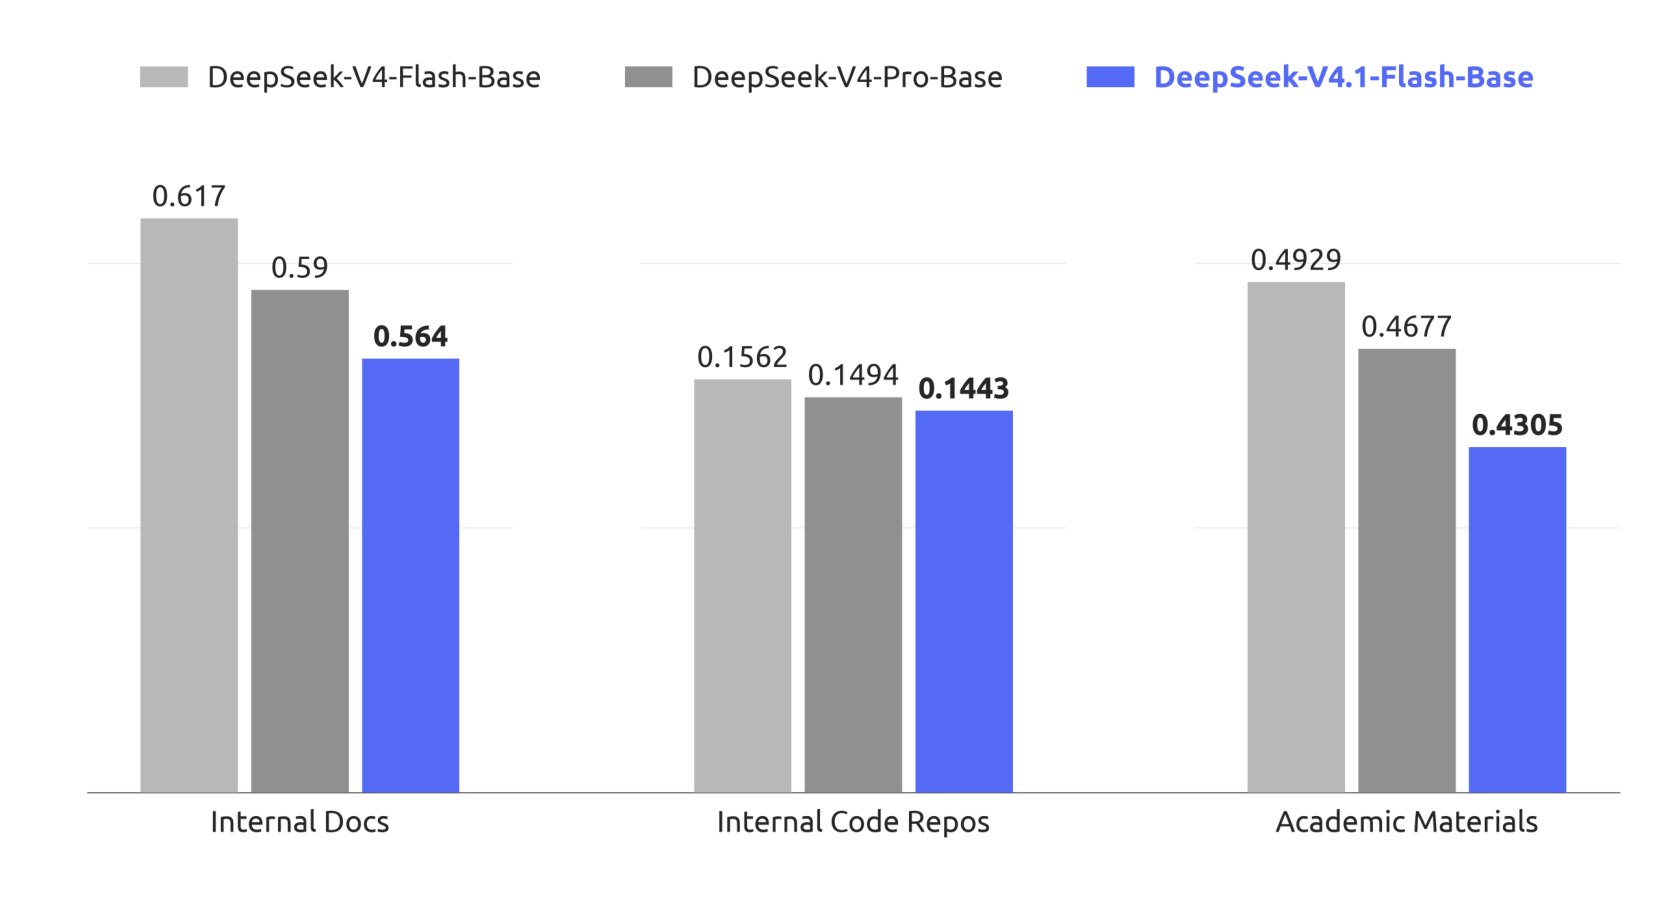
\includegraphics[width=\linewidth]{images_hi/fig06}
\caption{DeepSeek-V4-Flash-Base、DeepSeek-V4-Pro-Base 与 DeepSeek-V4.1-Flash-Base 在我们留出的评测集上的字节级困惑度（bits-per-byte, BPB）对比。DeepSeek-V4.1-Flash-Base 在所有任务上取得最低的 BPB，展现出作为强基础模型（base-model）的更大潜力。}
\label{fig:6}
\end{figure}